\documentclass{article}
\usepackage[final]{neurips_2019}

\usepackage[utf8]{inputenc} % allow utf-8 input
\usepackage[T1]{fontenc}    % use 8-bit T1 fonts
\usepackage{hyperref}       % hyperlinks
\usepackage{url}            % simple URL typesetting
\usepackage{booktabs}       % professional-quality tables
\usepackage{amsfonts}       % blackboard math symbols
\usepackage{nicefrac}       % compact symbols for 1/2, etc.
\usepackage{microtype}      % microtypography
\usepackage{amsmath}
\usepackage{graphicx}
\usepackage{subfigure}
\title{Exeriese 3}

\author{%
  Lan Zhang\\
  954517477\\
}

\begin{document}
\maketitle

\section{Problem 1}

Solved on 09/30/2019. The seed I used in bellowing experiments is 2612. 

I implemented ACC, BWT, TBWT, and CBWT to compare the result with different factors, including loss function, dropout, network depth, and optimizer. ACC measures mean performance through all tasks; BWT is the influence on task $T_i$ after the model trained on other tasks; TBWT set an independent standard for different tasks and calculate the influence on task $T_i$ after training other tasks; CBWT examines a specific task's influence.

$$ACC = \frac{1}{T}\sum_{i=1}^TR_{T,i}$$
$$BWT = \frac{1}{T-1}\sum_{i=1}^{T-1}R_{T,i}-R_{i,i}$$
$$TBWT = \frac{1}{T-1}\sum_{i=1}^{T-1}R_{T,i}-G_{i,i}$$
$$CBWT(t) = \frac{1}{T-t}\sum_{i=t+1}^{T}R_{i,t}-R_{t,t}$$
where $T$ is the total tasks in one experiment, $R_{i, j}$ is the performace(classification accuracy) of the model on task i after traning on task j, $G_{i, i}$ is the performance of a model only trained on task i.

Each experiment has 10 tasks. I applied a fixed random permutation to the pixels to generate different images as new tasks. Figure \ref{permutation} is an example of permutating images.  

\begin{figure}[htbp]
\centering
\subfigure[Original images]{
  \begin{minipage}{0.4\linewidth}
  \centering
  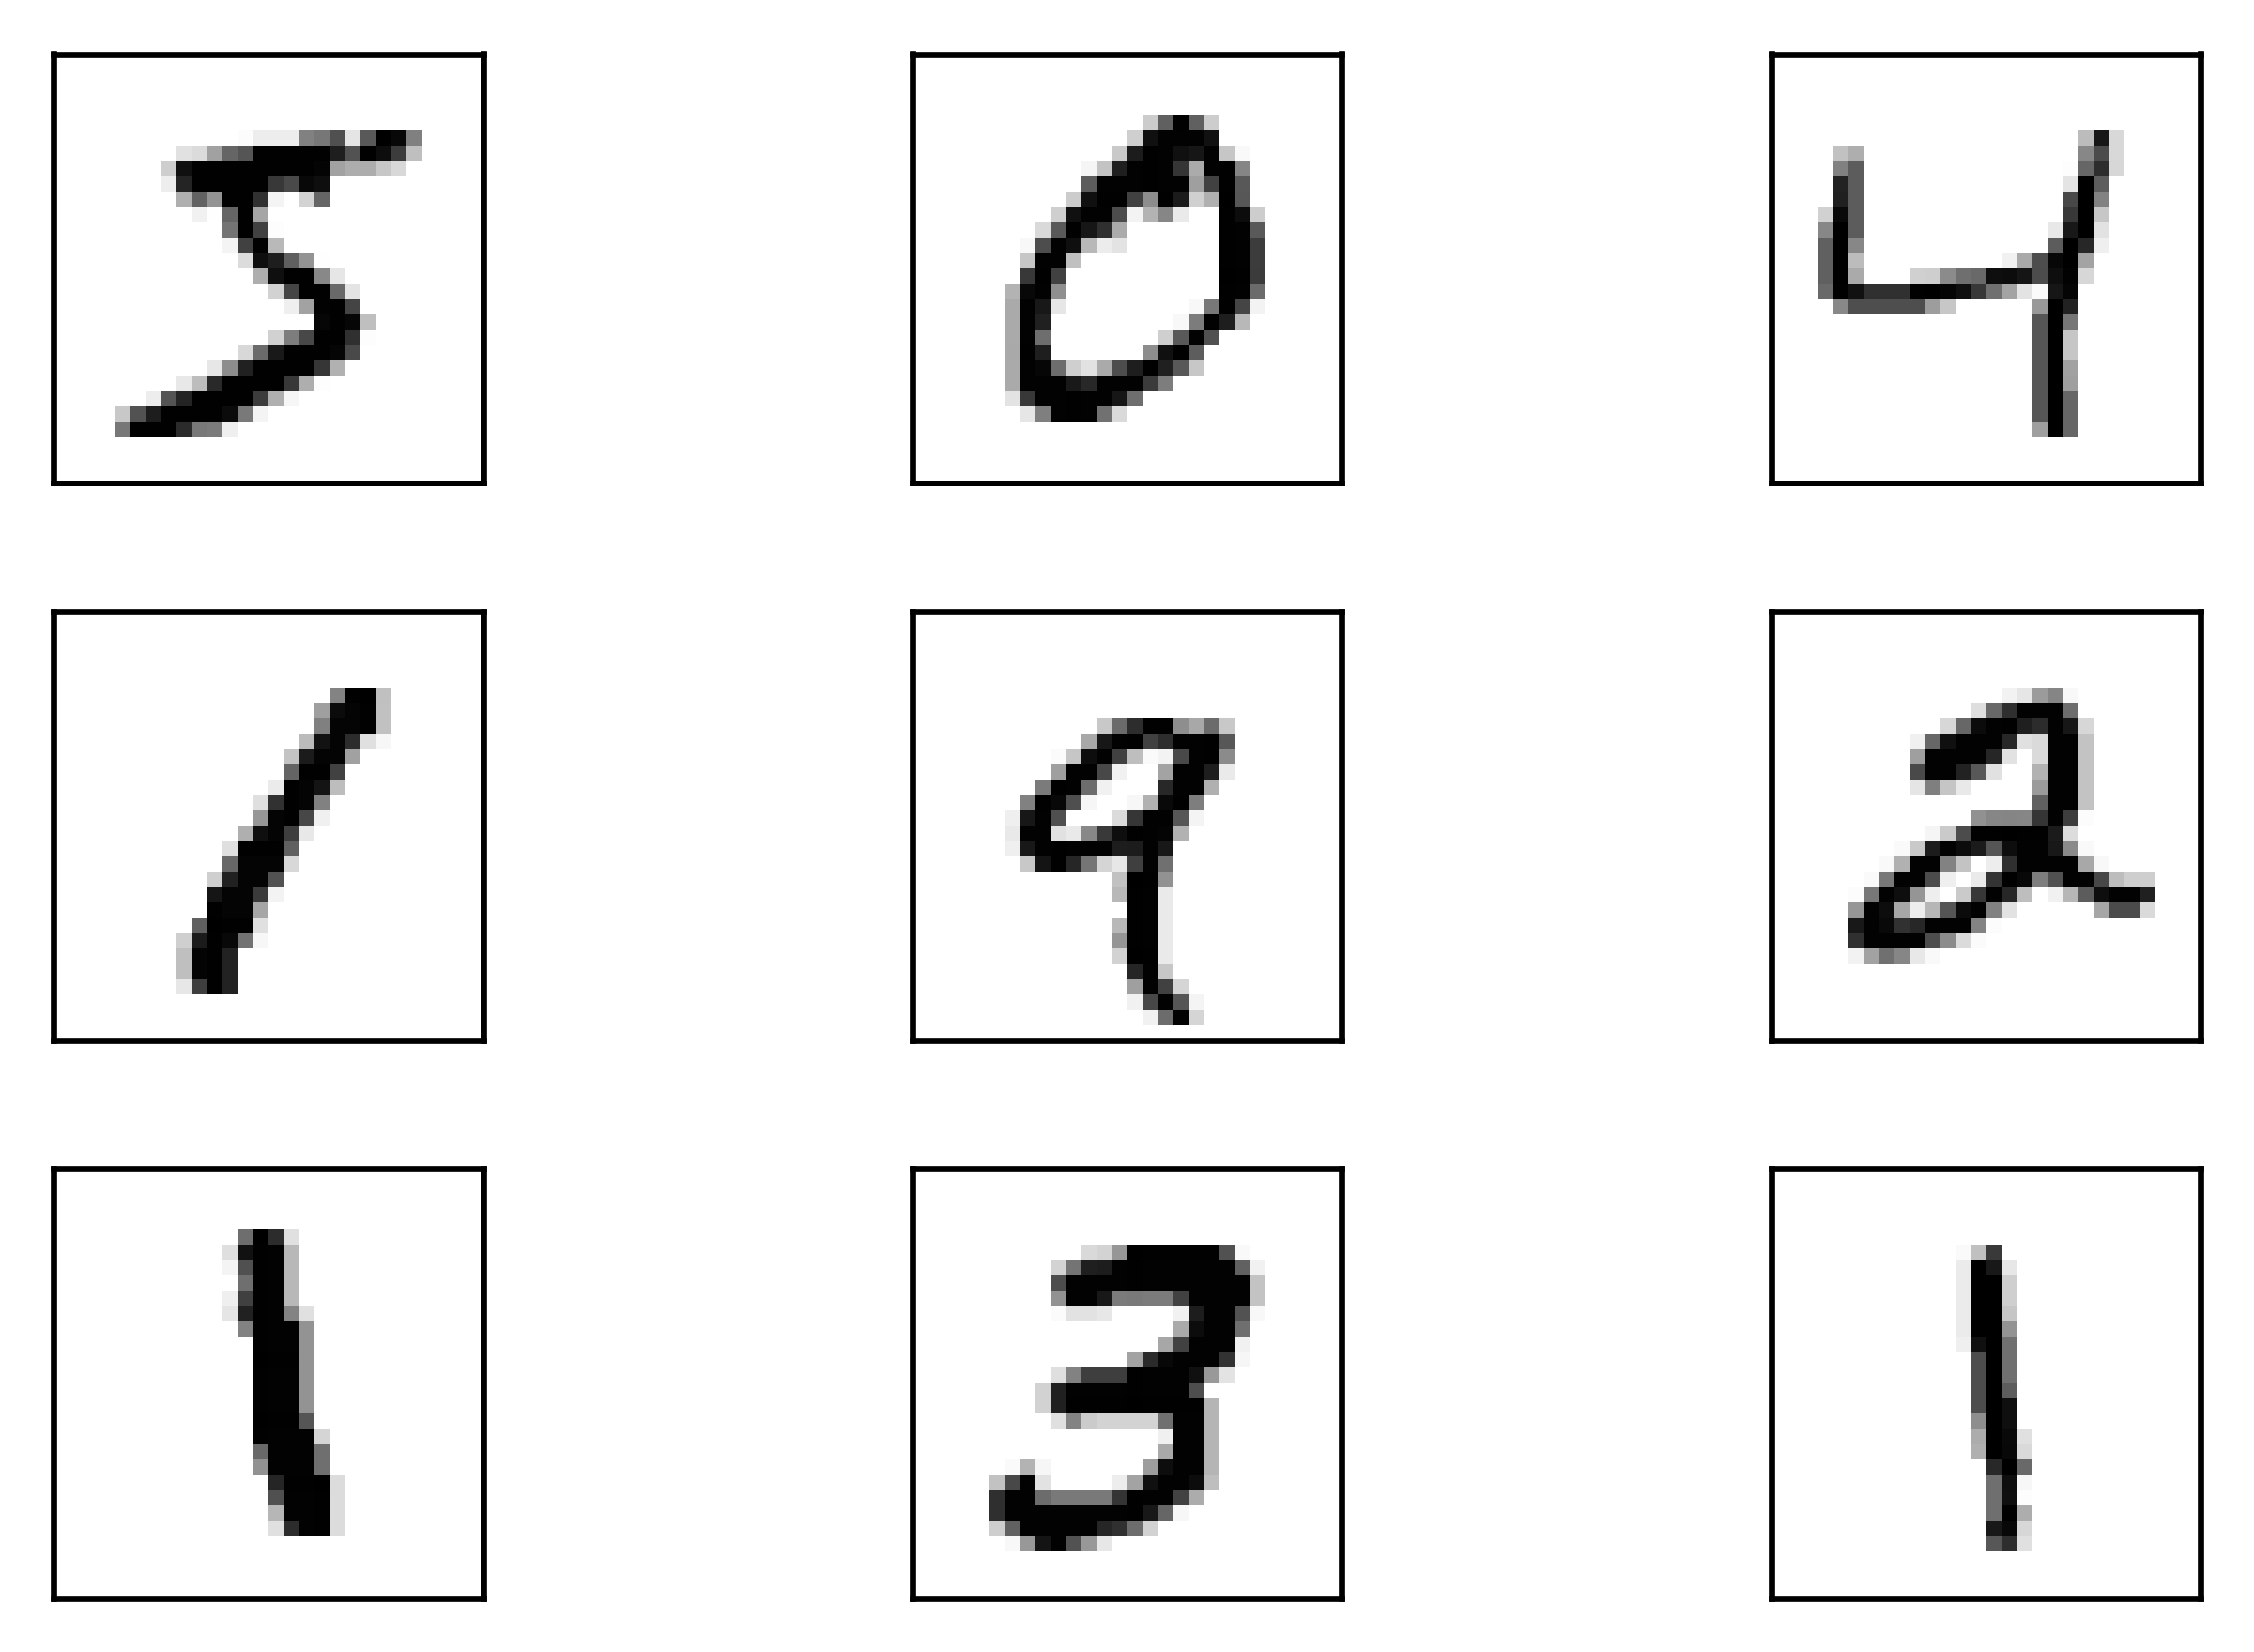
\includegraphics[scale=0.4]{img/index.png}
  \end{minipage}
}
\quad
\quad
\subfigure[Permuted images]{
\begin{minipage}{0.4\linewidth}
\centering
  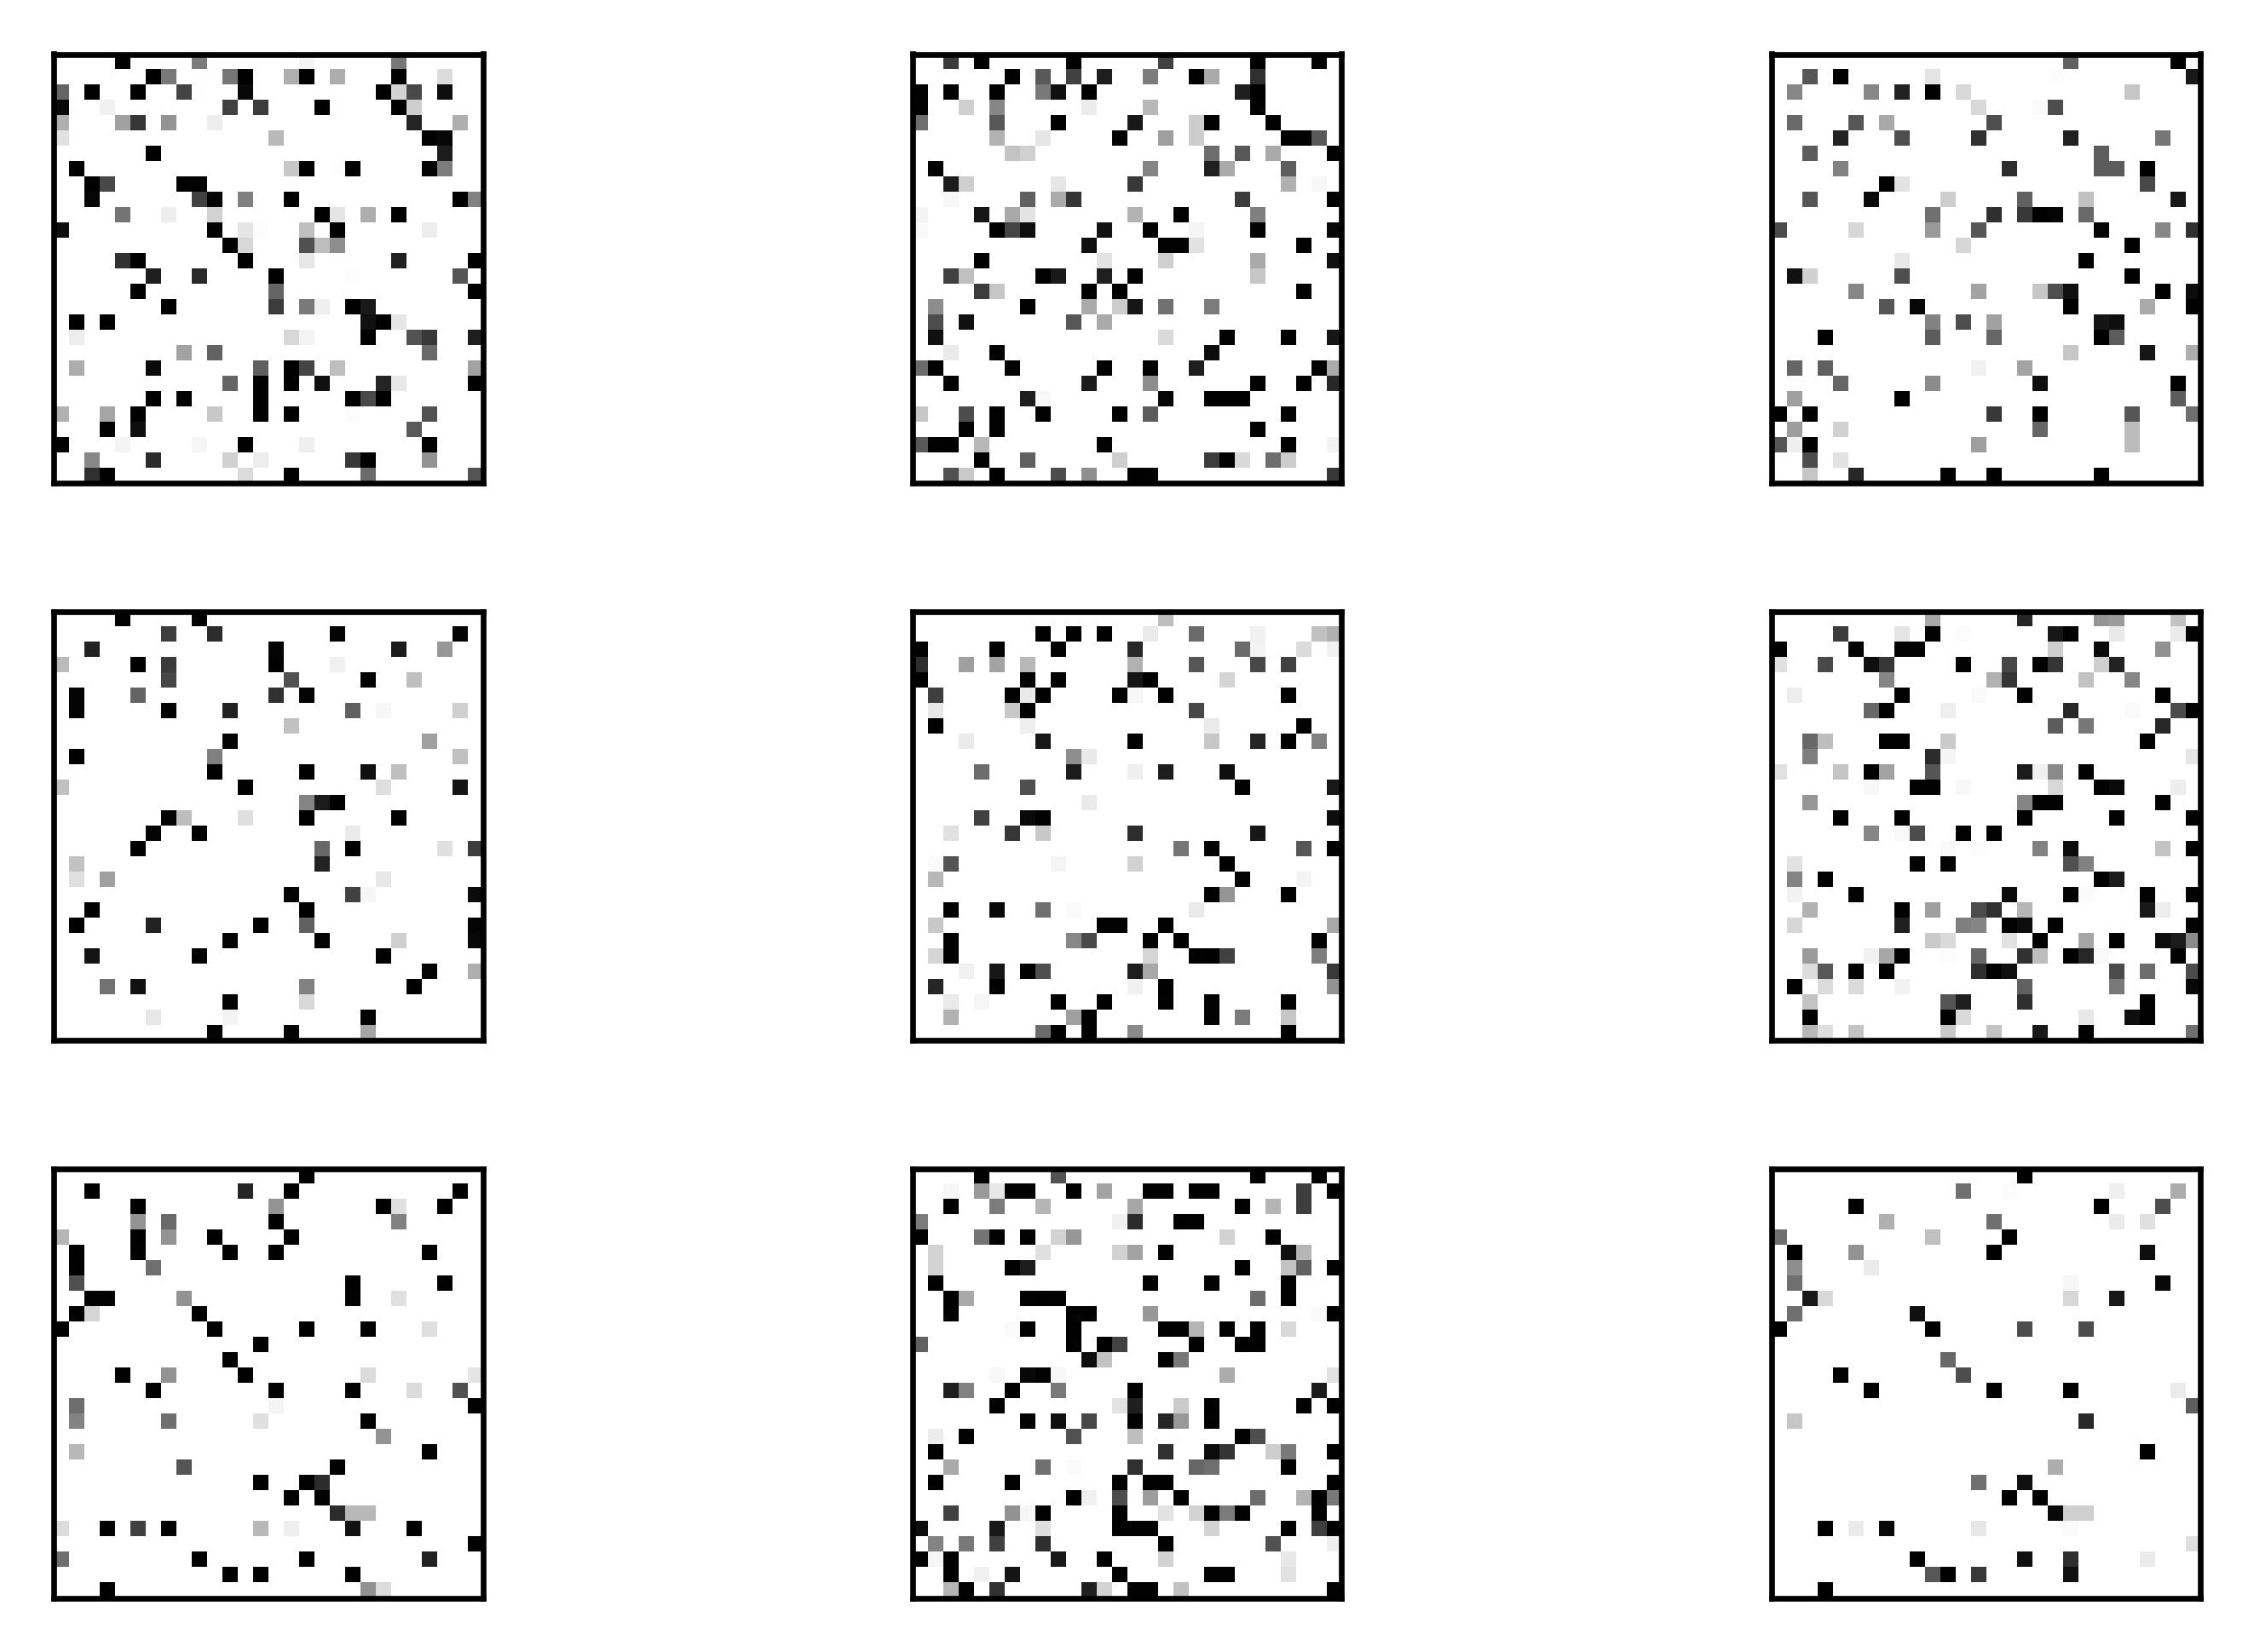
\includegraphics[scale=0.4]{img/permutation.png}
  \end{minipage}
}
\caption{Permutation}
\label{permutation}
\end{figure}

\subsection{Loss Function}
I implemented four loss function. The formula of Negative Log-Likelihodd(NLL) is:

$$NLL\_Loss(\hat{y}) = -log(\hat{y})$$

where $\hat{y}$ is the predicted class of the model.

I implemented L1 loss, L2 Loss and a hybird loss.
$$L1\_Loss(y, \hat{y}) = |\hat{y} - y|$$
$$L2\_Loss(y, \hat{y}) = \sqrt{(\hat{y} - y)^2}$$
$$Hybird\_Loss = (y, \hat{y}) =  L1\_Loss(y, \hat{y}) + L2\_Loss(y, \hat{y}) $$

Figure \ref{loss} is the four matrix with different loss function. Obviously, different loss functions influence the model of forgetting. L1 loss is better on resisting forgetting compared to other loss function s on this model.

\begin{figure}[htbp]
\centering
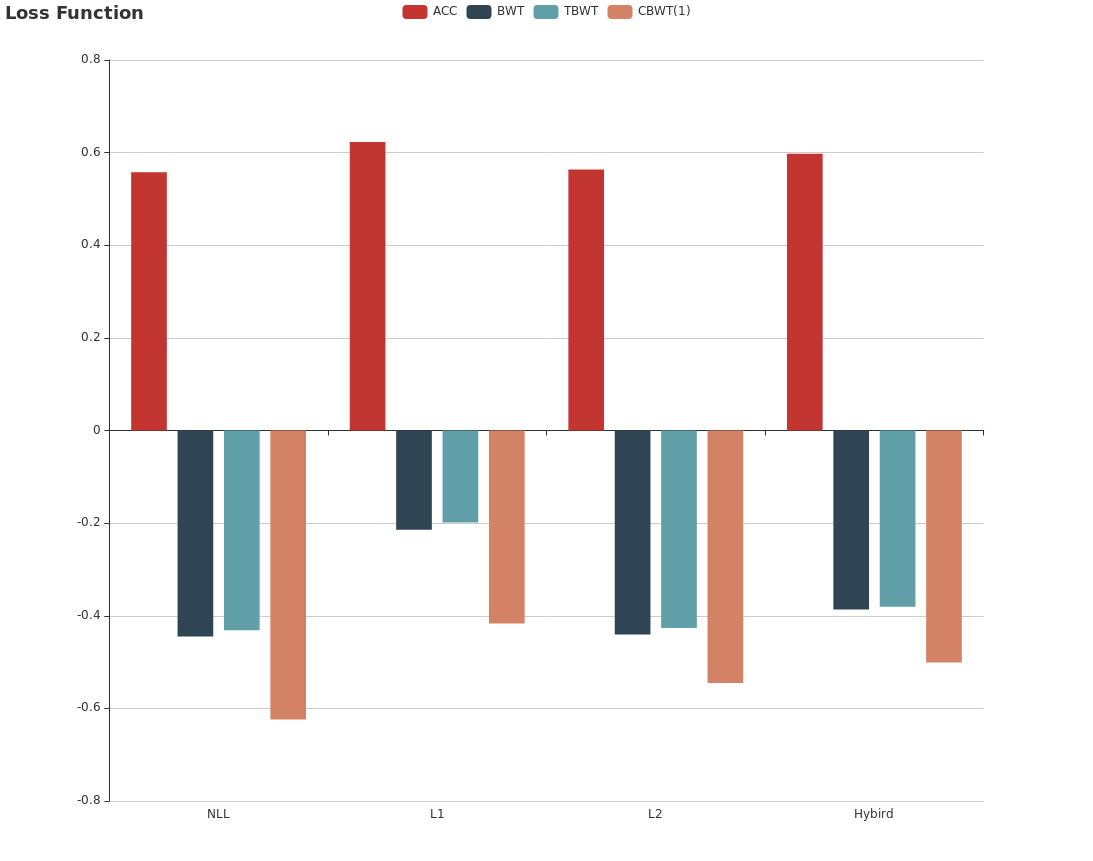
\includegraphics[scale=0.3]{img/LossFunction.png}
\caption{Loss Function}
\label{loss}
\end{figure}

\begin{figure}[htbp]
\centering
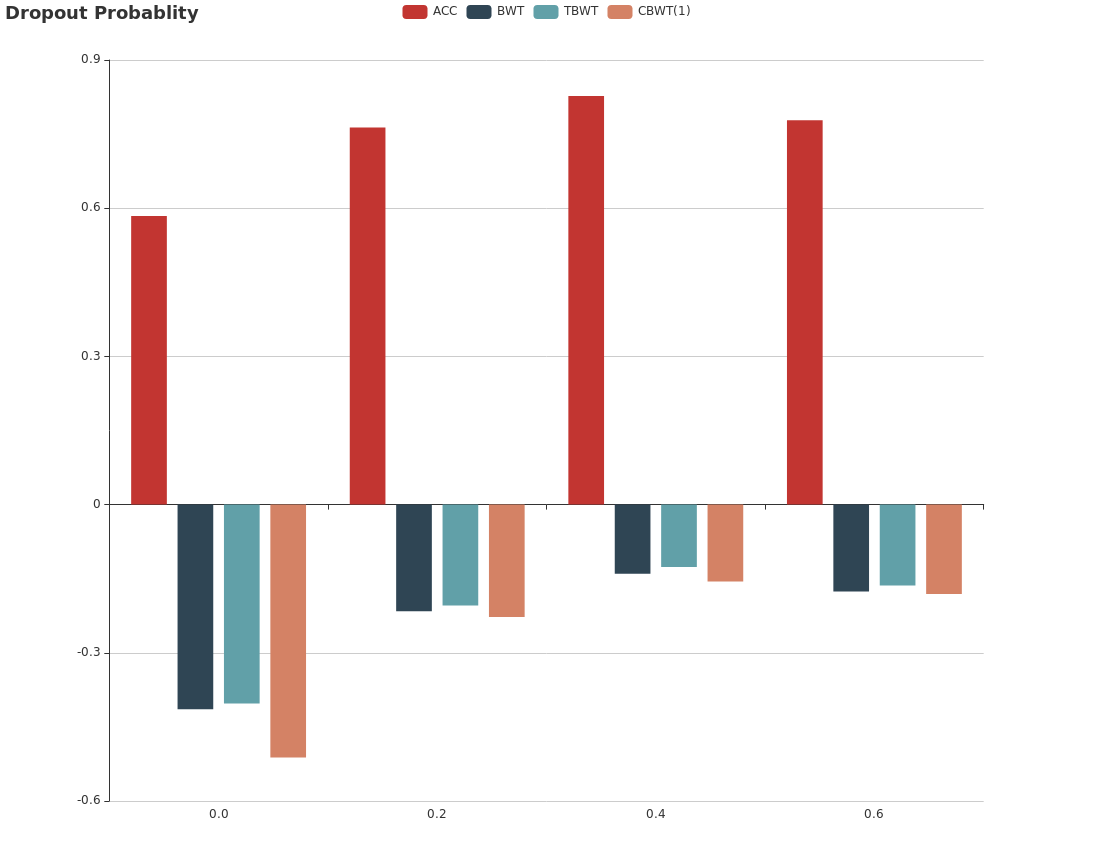
\includegraphics[scale=0.3]{img/DropoutProbablity.png}
\caption{Dropout Probablity}
\label{dropout}
\end{figure}

\subsection{Dropout}
I trid four dropout probablity(0.0, 0.2, 0.4, 0.6) in this experiment. Figure \ref{dropout} illustrates a large dropout probablity can reduce forgetting influence. That means if the model see more data on one task, it tends to forget more information after training on the future task.


\subsection{Depth}
I tried three models with different depth(2,3,4) in this experiment. Shown in Figure \ref{depth}, the more complex the model is, the larger the information loss has. I think it is because the complexity of the model affects the information it learn. I think that one of the reasons we use Occam'S razor rule when we choose models. 

\begin{figure}[htbp]
\centering
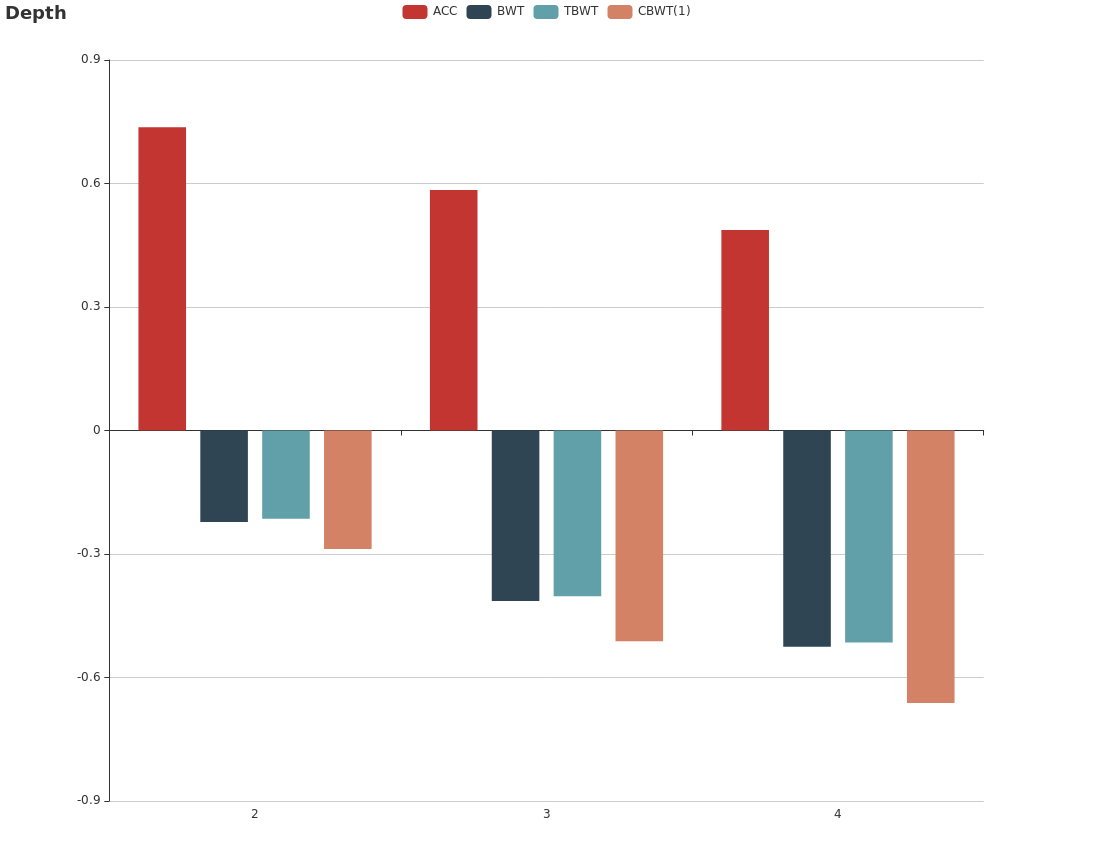
\includegraphics[scale=0.3]{img/Depth.png}
\caption{Depth}
\label{depth}
\end{figure}

\subsection{Optimizer}
I used three optimizers (Adam, SGD, RMSprop) with the same learning rate. Figure \ref{optimizer} is the result of this experiment. The model can't converge with the SGD optimizer. It seems optimizer doesn't affect as much as network depth and dropout probability on forgetting information.

\begin{figure}[htbp]
\centering
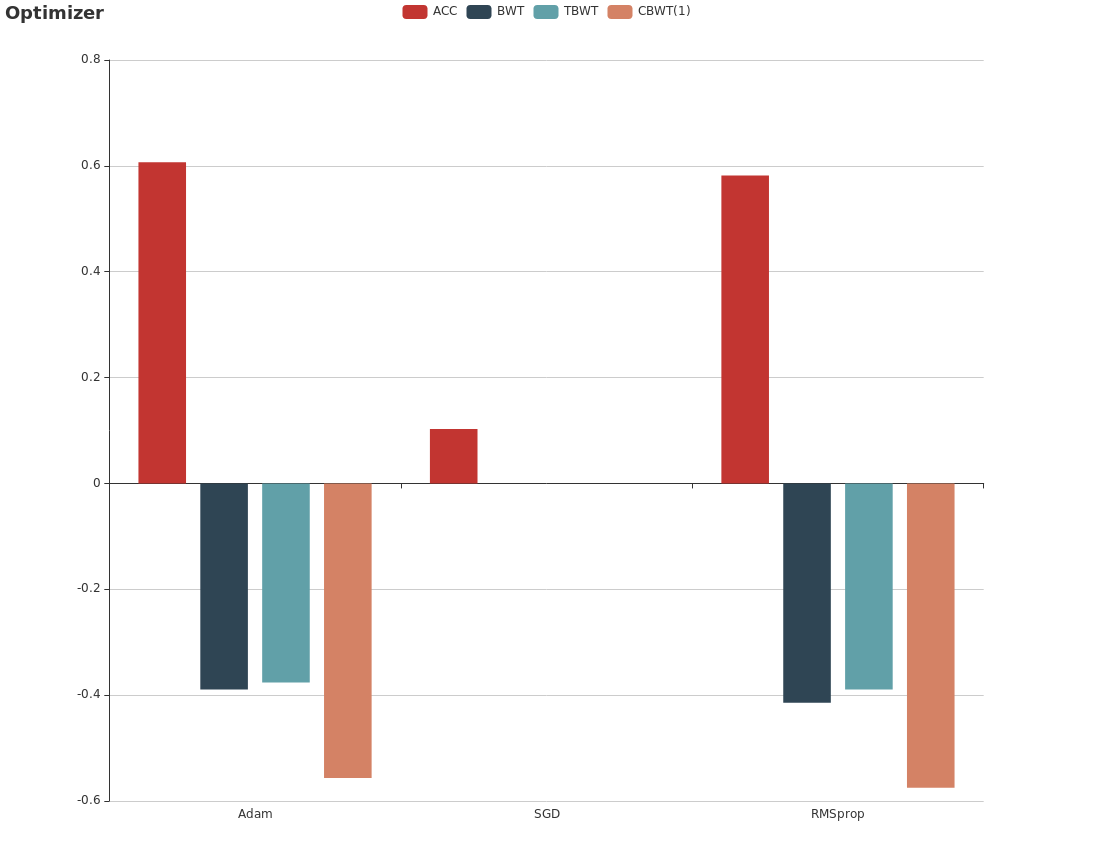
\includegraphics[scale=0.3]{img/Optimizer.png}
\caption{Optimizer}
\label{optimizer}
\end{figure}

\subsection{Validation Results}
Figure \ref{val} shows the accuracy and loss of the original test dataset during training 10 tasks. With more epochs on other tasks, the model is gradually forgetting information. The performance on original test dataset decreases sharply.


\begin{figure}[htbp]
\centering
\subfigure[Loss]{
  \begin{minipage}{0.4\linewidth}
  \centering
  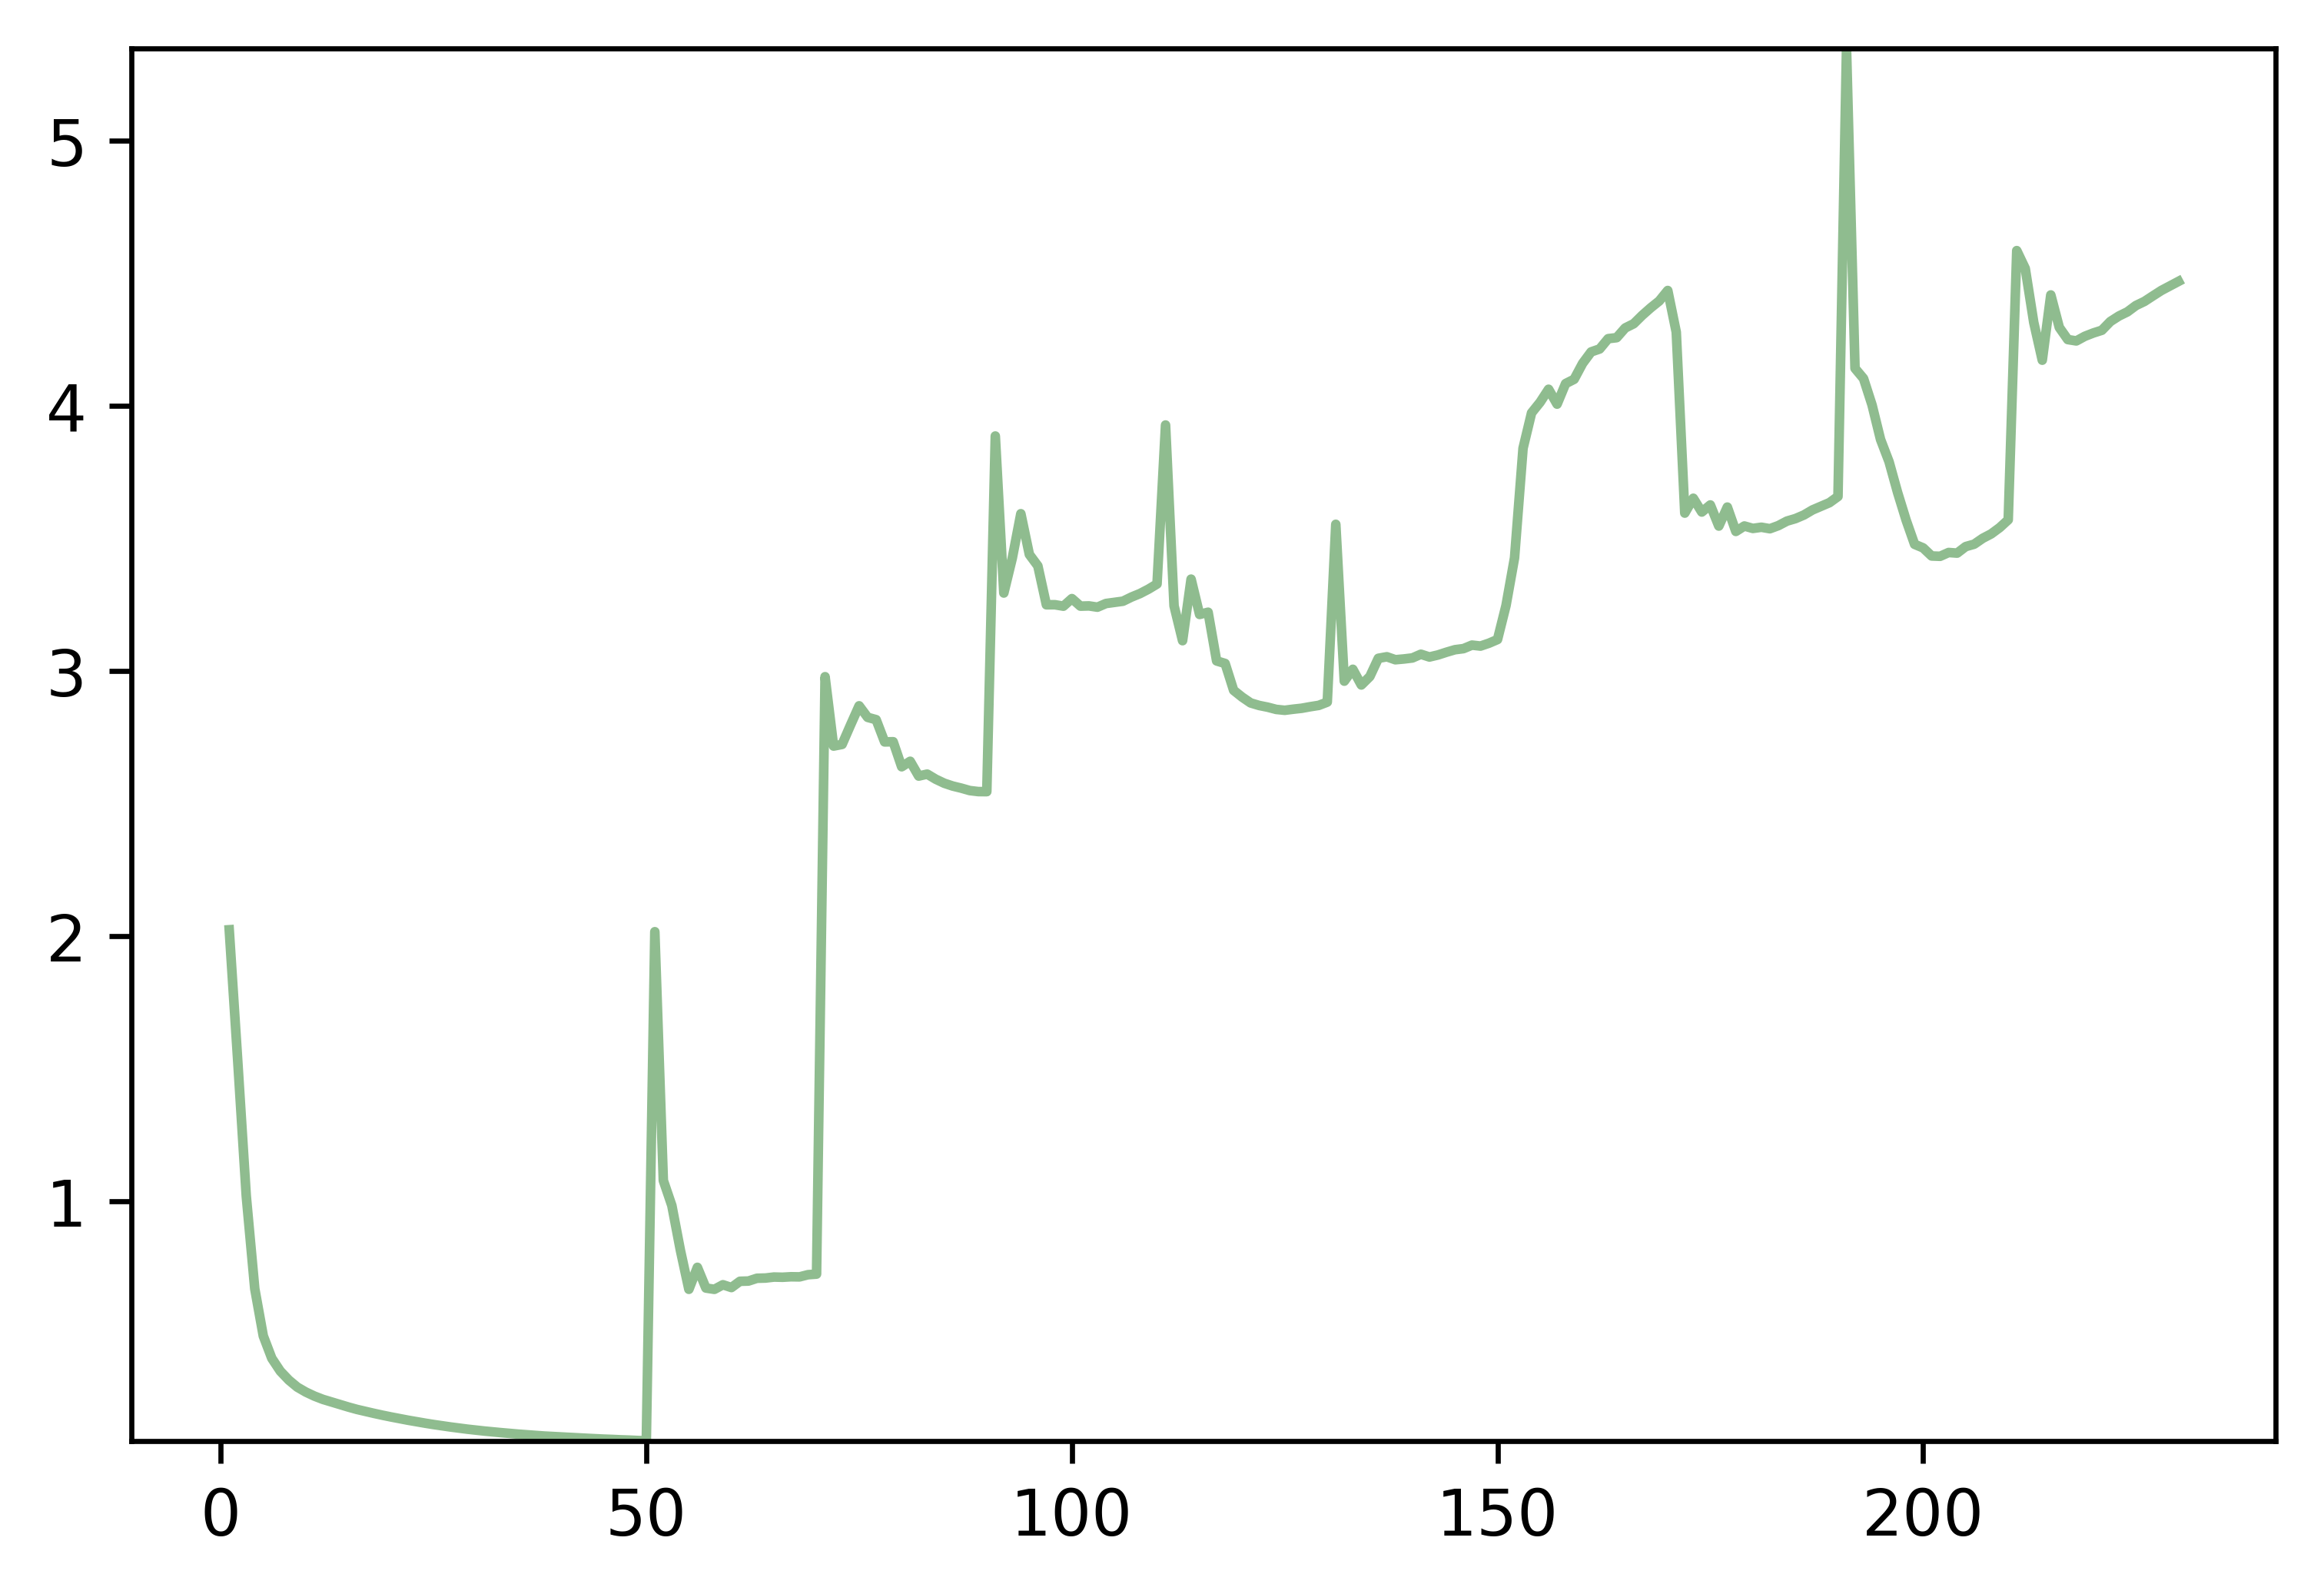
\includegraphics[scale=0.5]{img/loss.png}
  \end{minipage}
}
\quad
\quad
\subfigure[Accuracy]{
\begin{minipage}{0.4\linewidth}
\centering
  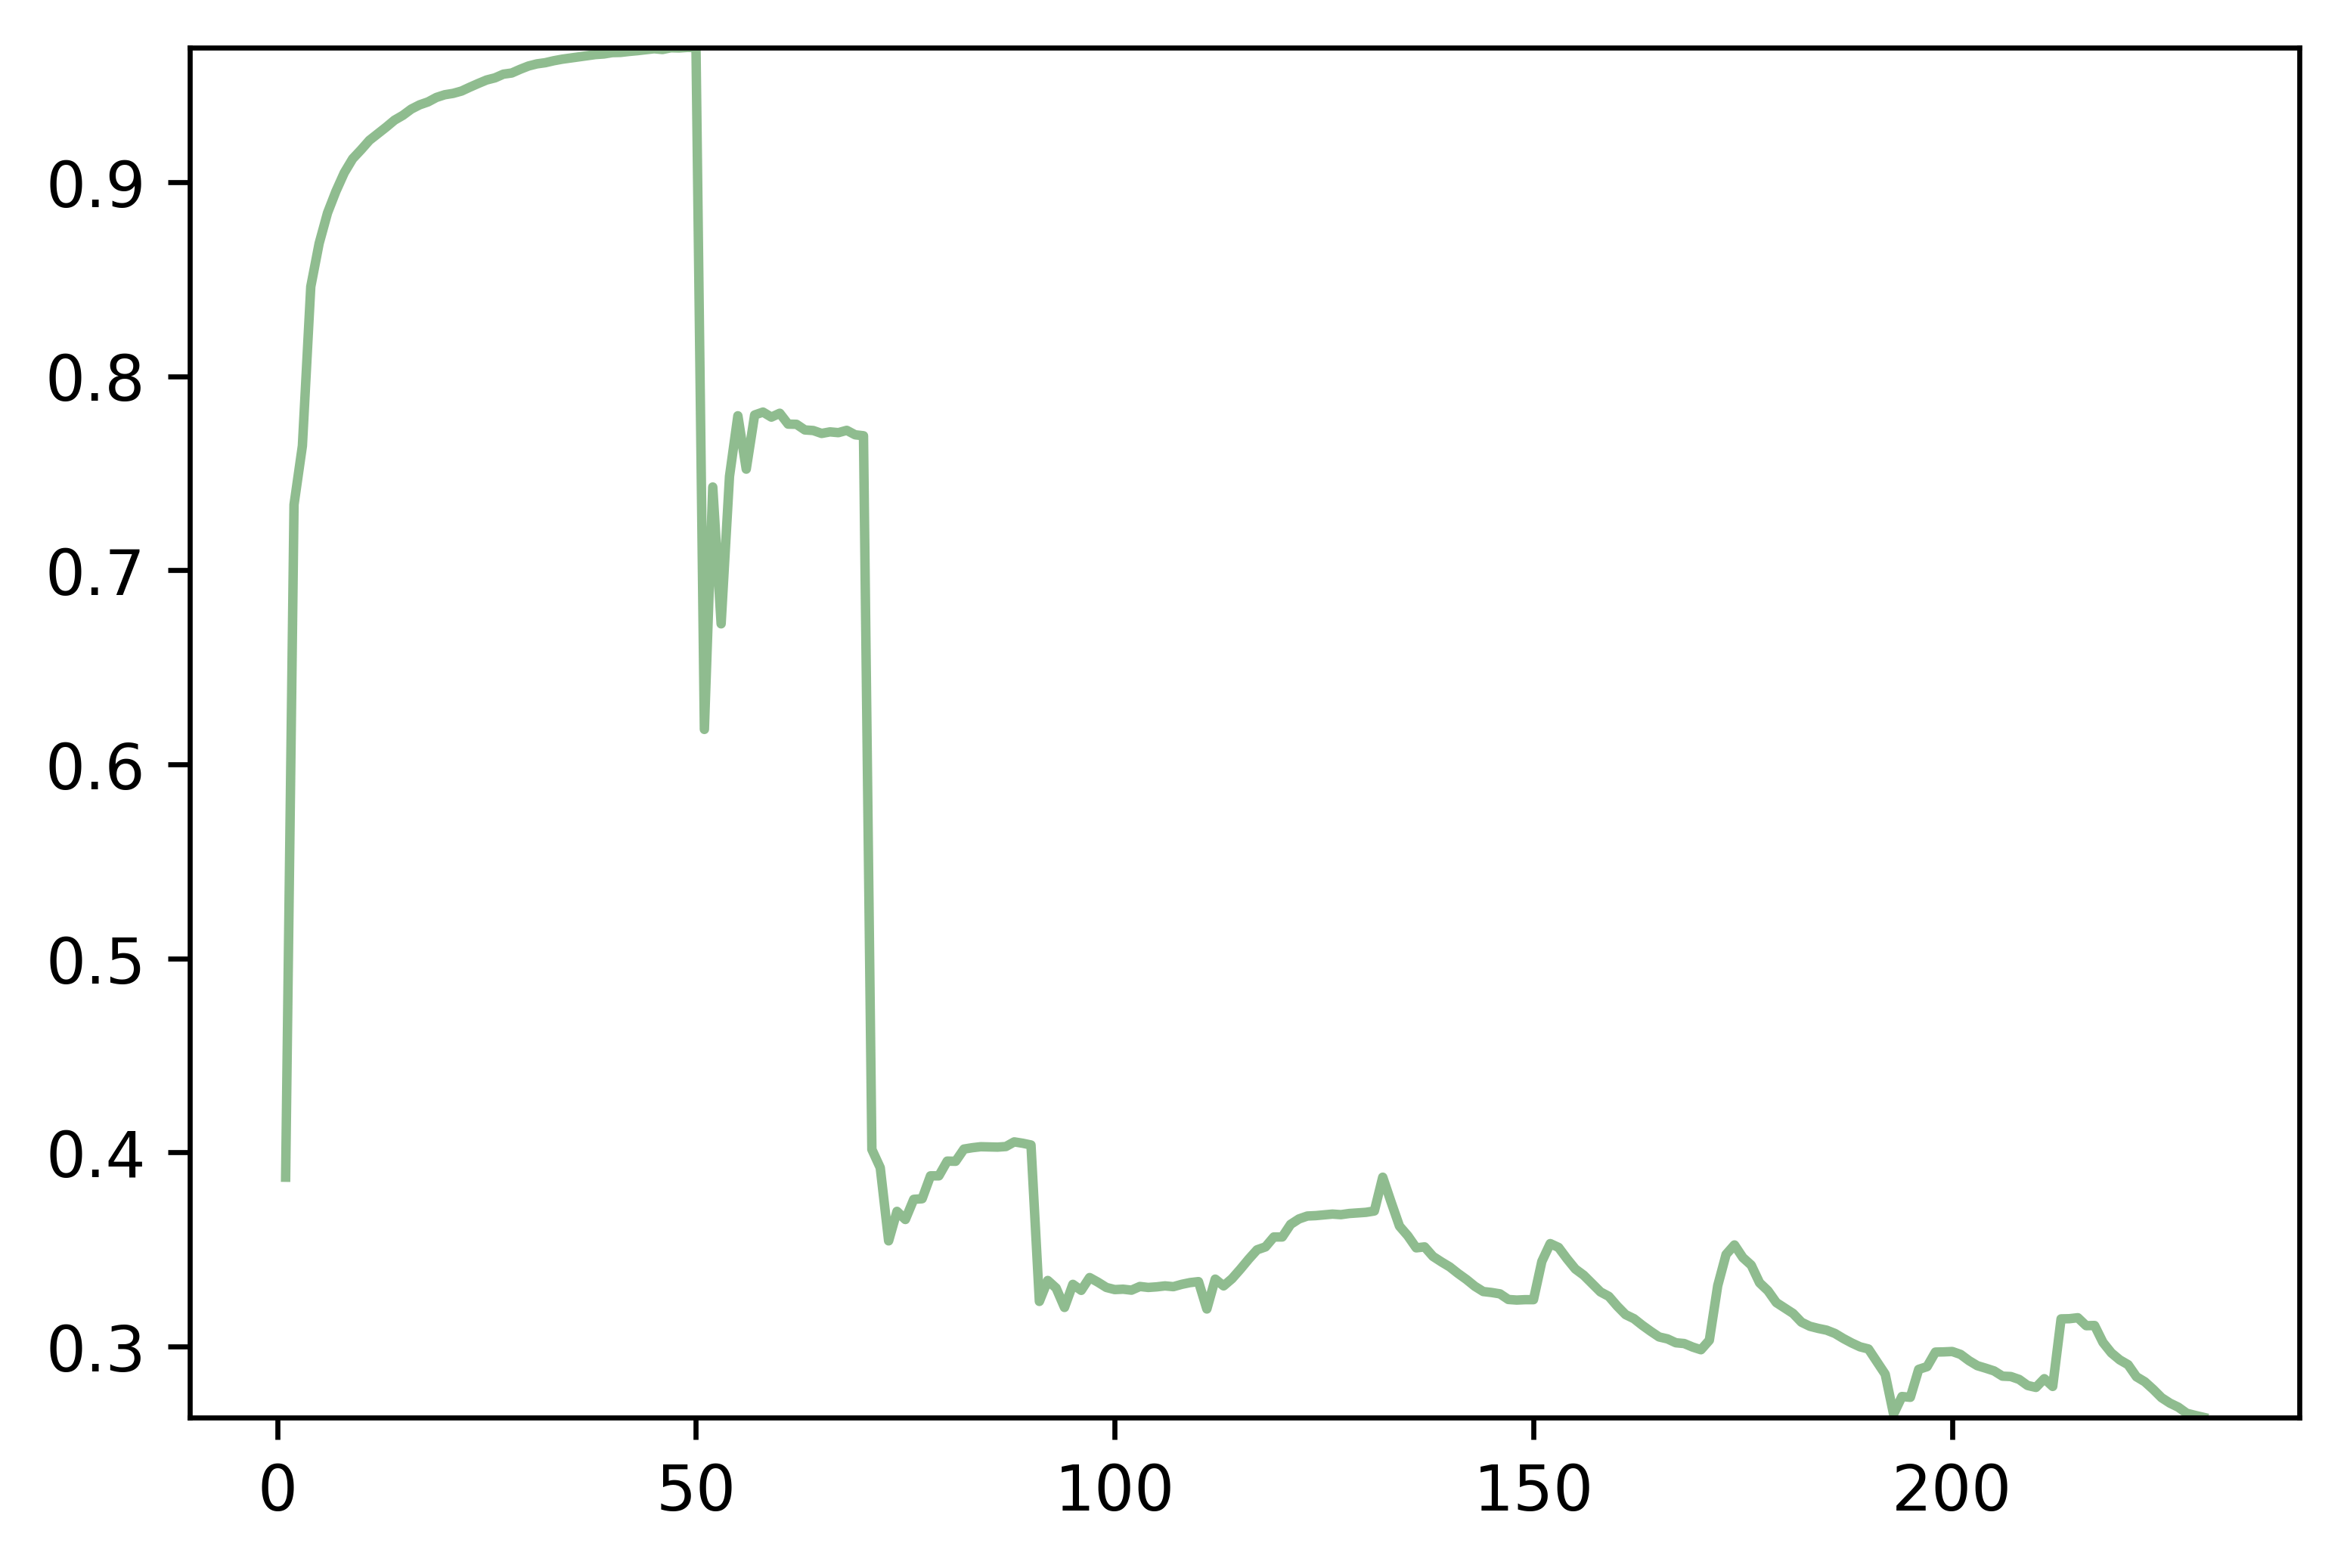
\includegraphics[scale=0.5]{img/acc.png}
  \end{minipage}
}
\caption{Validation Results}
\label{val}
\end{figure}

\end{document}
